\documentclass{article}
\usepackage[russian]{babel}
\usepackage[utf8]{inputenc}
\usepackage[T2]{fontenc}
\usepackage{graphicx}
\graphicspath{ {images/} }

\title{ТМП ДЗ №1}
\author{Максим Щемилкин A-05-19}
\date{30 марта 2022}

\begin{document}
\maketitle
\section{Построить конечный автомат, распознающий язык}


    \quad 1. $L = \{w \in \{a, b, c\}^*\quad|w|_c = 1\}$
    \begin{center}
        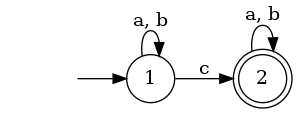
\includegraphics[width=0.4\textwidth]{pic1.dot}
    \end{center}
    \quad 2. $L = \{w \in \{a, b\}^* \quad |w|_a \leq 2, |w|_b \geq 2\}$
    \begin{center}
        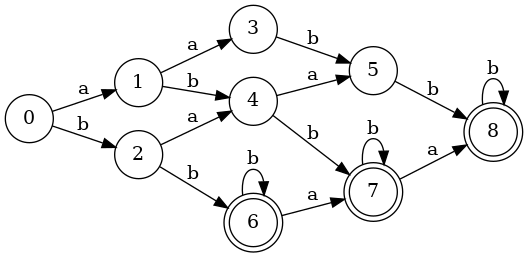
\includegraphics[width=0.8\textwidth]{pic2.dot}\\
    \end{center}
    Это решение получается через перебор первых 4 символов. Такой же результат можно получить через произведение двух грамматик:\\
    $$L_1 = \{w \in \{a, b\}^* \quad |w|_a \leq 2\}, \quad L_2 = \{w \in \{a, b\}^* \quad |w|_b \geq 2\}$$\\
    \begin{center}
        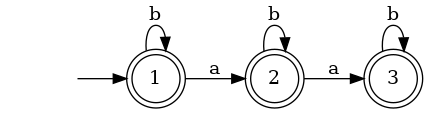
\includegraphics[width=0.45\textwidth]{pic3.dot}
        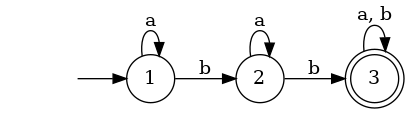
\includegraphics[width=0.45\textwidth]{pic4.dot}
    \end{center}
    \begin{center}
        \begin{tabular}{|c|c|c|}
            \hline
            Сочетания точек & По А & По В \\
            \hline
            11 & 21 & 12\\
            12 & 22 & 13\\
            13 & 23 & 13\\
            21 & 31 & 22\\
            22 & 32 & 23\\
            23 & 33 & 23\\
            31 &  & 32\\
            32 &  & 33\\
            33 &  & 33\\
            \hline
        \end{tabular}\\
    \end{center}
    Получим:
    \begin{center}
        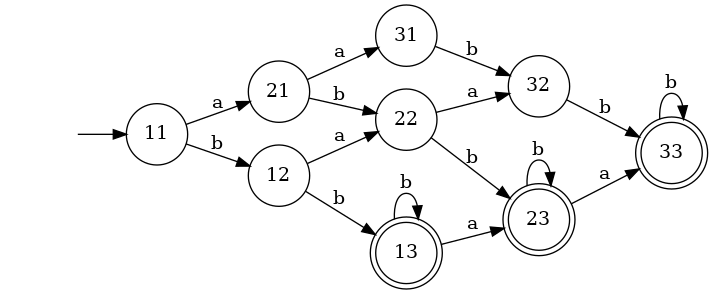
\includegraphics[width=0.9\textwidth]{pic5.dot}\\
    \end{center}
    \quad 3. $L = \{w \in \{a, b\}^* \quad |w|_a \neq |w|_b\}$
    \begin{center}
        Нет такого конечного автомата
    \end{center}
    \quad 4. $L = \{w \in \{a, b\}^* \quad ww = www\}$\\
    Это возможно только для языка, состоящего из пустого слова, так как при $|w|>0 ww \neq www$. Можем построить недерминированный КА:
    \begin{center}
        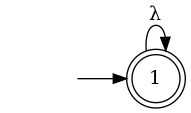
\includegraphics[width=0.3\textwidth]{pic6.dot}\\
    \end{center}
    
\section{Построить КА, используя прямое произведение}

    1. $L_1 = \{w \in \{a, b\}^* \quad |w|_a \geq 2 \wedge |w|_b \geq 2\}$\\
    Разобьем на 2 автомата:
    $$L_11 = \{w \in \{a, b\}^* \quad |w|_a \geq 2\}, \quad L_12 = \{w \in \{a, b\}^* \quad |w|_b \geq 2\}$$\\
    \begin{center}
        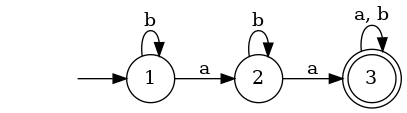
\includegraphics[width=0.45\textwidth]{pic7.dot}
        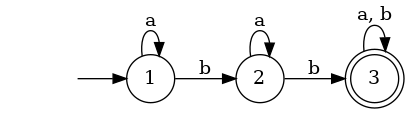
\includegraphics[width=0.45\textwidth]{pic4.dot}
    \end{center}
    Значит, $L = L_11 \wedge L_12$. Имеем $\Sigma = {a, b}, s = 11, T = 33$. Зафиксируем переходы между новыми вершинами:
    \begin{center}
        \begin{tabular}{|c|c|c|}
            \hline
            Сочетания точек & По А & По В \\
            \hline
            11 & 21 & 12\\
            12 & 22 & 13\\
            13 & 23 & 13\\
            21 & 31 & 22\\
            22 & 32 & 23\\
            23 & 33 & 23\\
            31 & 31 & 32\\
            32 & 32 & 33\\
            33 & 33 & 33\\
            \hline
        \end{tabular}\\
    \end{center}
    Получим:
    \begin{center}
        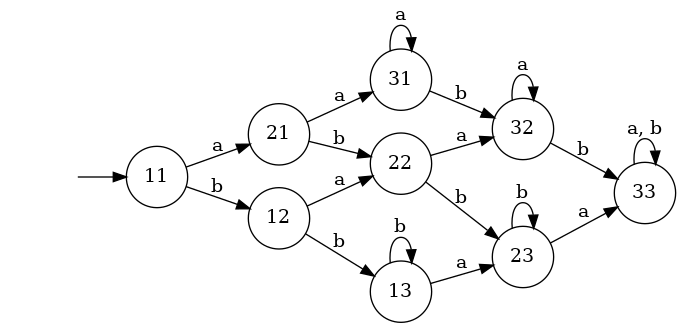
\includegraphics[width=0.9\textwidth]{pic8.dot}\\
    \end{center}
    
    2. $L_2 = \{w \in \{a, b\}^* \quad |w| \geq 3 \wedge |w|\quad odd\}$\\
    Разобьем на 2 автомата:
    $$L_21 = \{w \in \{a, b\}^* \quad |w| \geq 3\}, \quad L_22 = \{w \in \{a, b\}^* \quad |w|\quad odd\}$$
    \begin{center}
        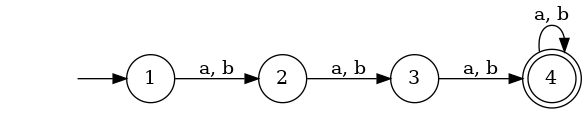
\includegraphics[width=0.6\textwidth]{pic9.dot}
        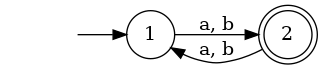
\includegraphics[width=0.3\textwidth]{pic10.dot}
    \end{center}
    Значит, $L = L_21 \wedge L_22$. Имеем $\Sigma = {a, b}, s = 11, T = 42$. Зафиксируем переходы между новыми вершинами:
    \begin{center}
        \begin{tabular}{|c|c|c|}
            \hline
            Сочетания точек & По А & По В \\
            \hline
            11 & 22 & 22\\
            12 & 21 & 21\\
            21 & 32 & 32\\
            22 & 31 & 31\\
            31 & 42 & 42\\
            32 & 41 & 41\\
            41 & 42 & 42\\
            42 & 41 & 41\\
            \hline
        \end{tabular}\\
    \end{center}
    Получим:
    \begin{center}
        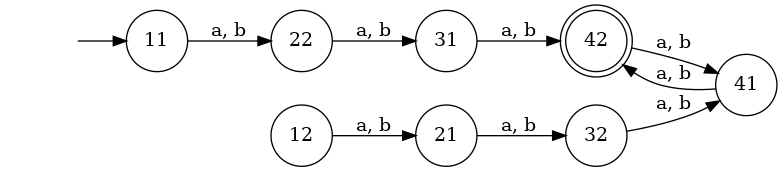
\includegraphics[width=0.9\textwidth]{pic11.dot}\\
    \end{center}
    Так как в вершину 12 попасть нельзя, можно автомат немного упростить:
    \begin{center}
        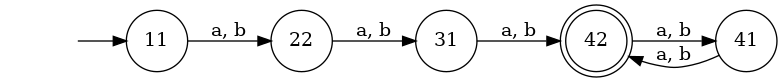
\includegraphics[width=0.9\textwidth]{pic12.dot}\\
    \end{center}
    
    3. $L_3 = \{w \in \{a, b\}^* \quad |w|_a\, \vdots\, 2 \wedge |w|_b\, \vdots\, 3\}$\\
    Разобьем на 2 автомата:
    $$L_31 = \{w \in \{a, b\}^* \quad |w|_a\, \vdots\, 2\}, \quad L_32 = \{w \in \{a, b\}^* \quad |w|_b\, \vdots\, 3\}$$
    \begin{center}
        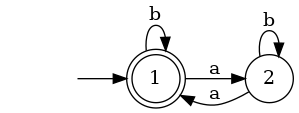
\includegraphics[width=0.4\textwidth]{pic13.dot}
        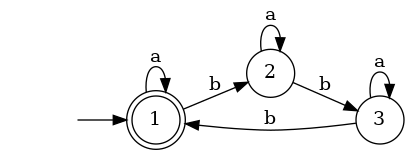
\includegraphics[width=0.5\textwidth]{pic14.dot}
    \end{center}
    Значит, $L = L_31 \wedge L_32$. Имеем $\Sigma = {a, b}, s = 11, T = 11$. Зафиксируем переходы между новыми вершинами:
    \begin{center}
        \begin{tabular}{|c|c|c|}
            \hline
            Сочетания точек & По А & По В \\
            \hline
            11 & 21 & 12\\
            12 & 22 & 13\\
            13 & 23 & 11\\
            21 & 11 & 22\\
            22 & 12 & 23\\
            23 & 13 & 21\\
            \hline
        \end{tabular}\\
    \end{center}
    Получим:
    \begin{center}
        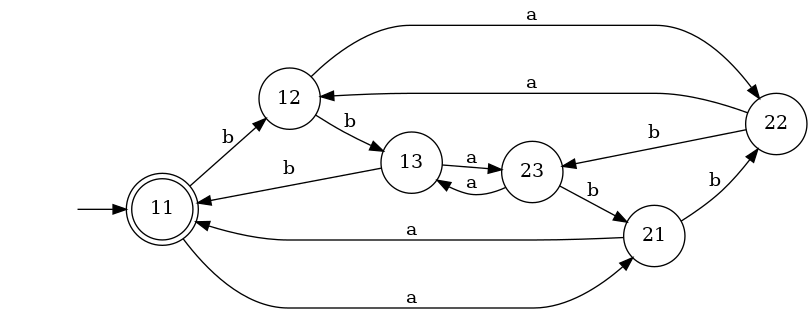
\includegraphics[width=0.9\textwidth]{pic15.dot}
    \end{center}
    
    
    4. $L_4 = \overline{L_3}$\\
    Чтобы построить отрицание, нужно обратить конечные вершины, то есть получим:
    \begin{center}
        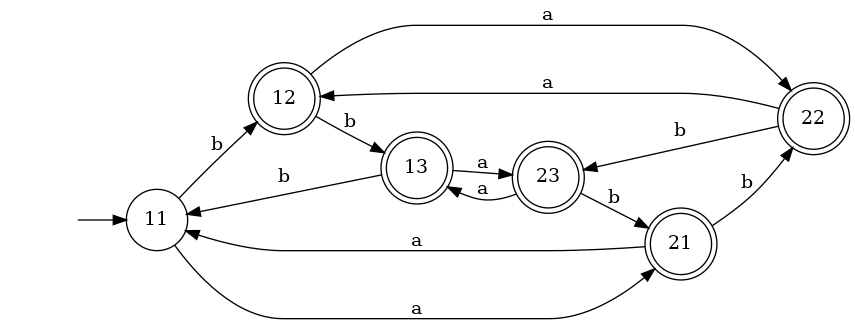
\includegraphics[width=0.9\textwidth]{pic16.dot}
    \end{center}
    
    5. $L_5 = L_2 \setminus L_3 = L_2 \wedge L_4 $\\
    Найдём пересечение двух языков:
    \begin{center}
        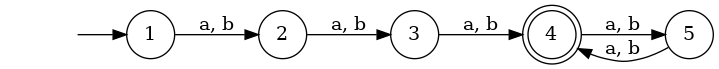
\includegraphics[width=0.9\textwidth]{pic2_5_1.dot}
        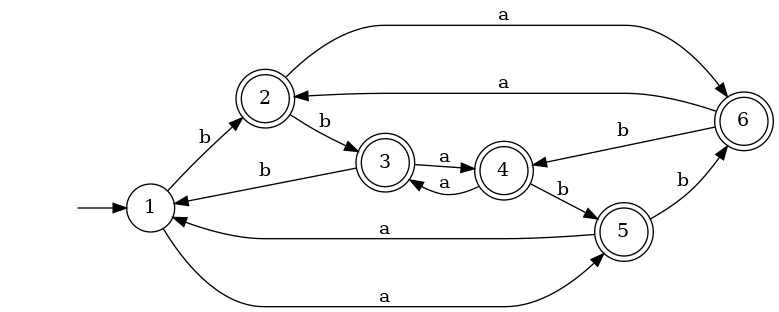
\includegraphics[width=0.9\textwidth]{pic2_5_2.dot}
    \end{center}
    $L_5 = L_2 \wedge L_4$. Имеем $\Sigma = \{a, b\}, s = 11, T = 42$. Зафиксируем переходы между новыми вершинами:
    \begin{center}
        \begin{tabular}{|c|c|c|}
            \hline
            Сочетания точек & По А & По В \\
            \hline
            11 & 25 & 22\\
            12 & 26 & 23\\
            13 & 24 & 21\\
            14 & 23 & 25\\
            15 & 21 & 26\\
            16 & 22 & 24\\
            21 & 35 & 32\\
            22 & 36 & 33\\
            23 & 34 & 31\\
            24 & 33 & 35\\
            25 & 31 & 36\\
            26 & 32 & 34\\
            31 & 45 & 42\\
            32 & 46 & 43\\
            33 & 44 & 41\\
            34 & 43 & 45\\
            35 & 41 & 46\\
            36 & 42 & 44\\
            41 & 55 & 52\\
            42 & 56 & 53\\
            43 & 54 & 51\\
            44 & 53 & 55\\
            45 & 51 & 56\\
            46 & 52 & 54\\
            51 & 45 & 62\\
            52 & 46 & 43\\
            53 & 44 & 41\\
            54 & 43 & 45\\
            55 & 41 & 46\\
            56 & 42 & 44\\
            \hline
        \end{tabular}\\
    \end{center}
    Получим:
    \begin{center}
        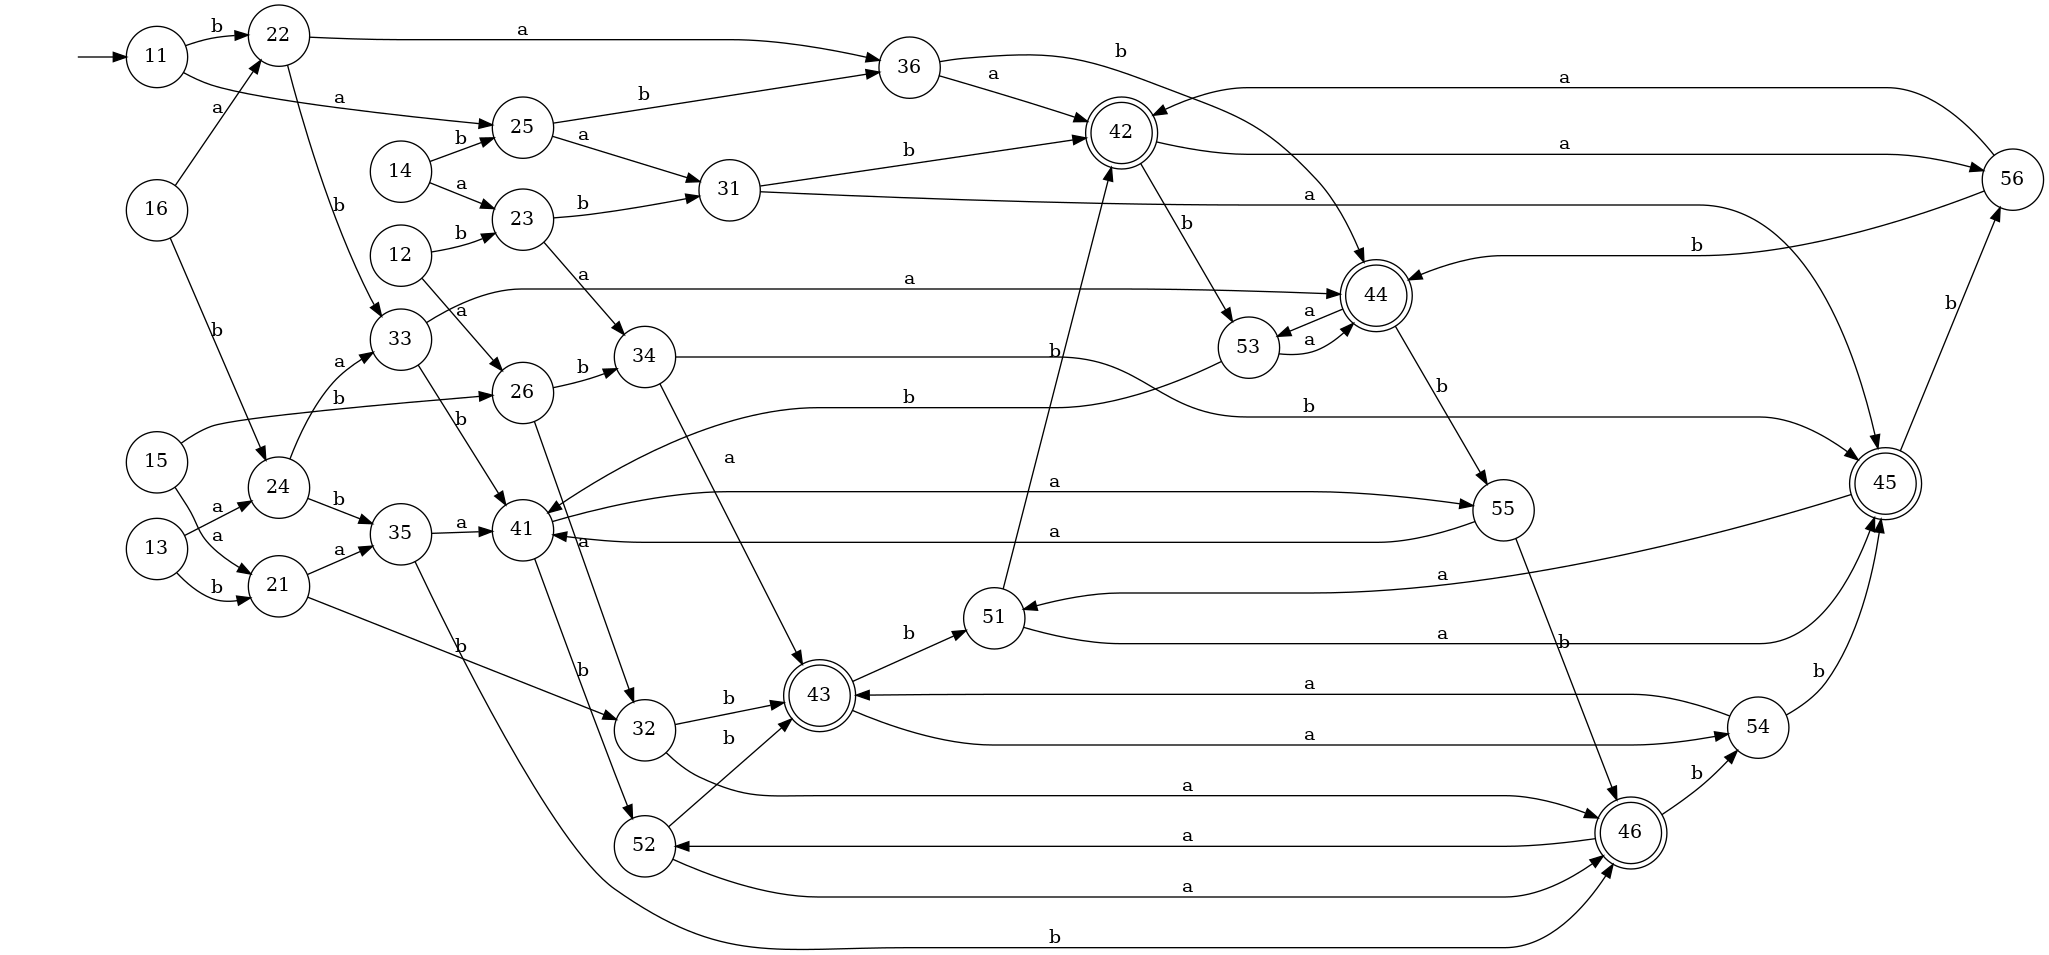
\includegraphics[width=1\textwidth]{pic2_5_3.dot}\\
    \end{center}
    
\section{Построить минимальный ДКА по регулярному выражению}
    1. $(ab+aba)^*a$\\
    Недетерминированный КА по данному выражению:
    \begin{center}
        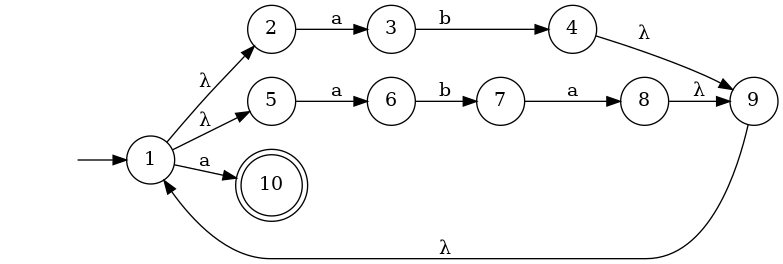
\includegraphics[width=1\textwidth]{pic3_1_1.dot}\\
    \end{center}
    \begin{center}
        \begin{tabular}{|c|c|c|}
            \hline
            Сочетания точек & По А & По В \\
            \hline
            1 & 3 6 10 & \\
            3 6 10 & & 4 7 \\
            4 7 & 8 3 6 10 & \\
            8 3 6 10 & 3 6 10 & 4 7\\
            \hline
        \end{tabular}\\
    \end{center}
    Теперь можем нарисовать ДКА:
    \begin{center}
        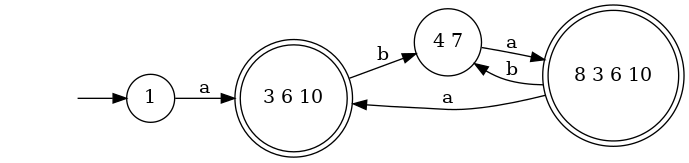
\includegraphics[width=1\textwidth]{pic3_1_2.dot}\\
    \end{center}
    
    2. $a(a(ab)^*b)^*(ab)^*$\\
    Недетерминированный КА по данному выражению:
    \begin{center}
        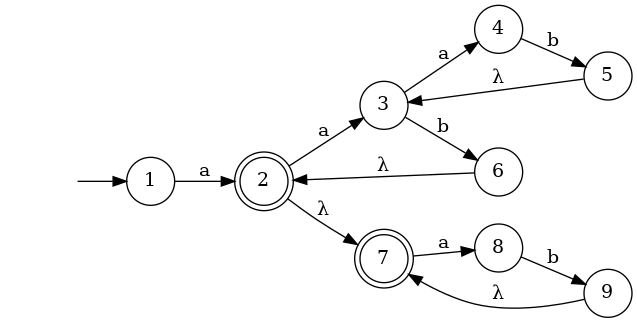
\includegraphics[width=1\textwidth]{pic3_2_1.dot}\\
    \end{center}
    \begin{center}
        \begin{tabular}{|c|c|c|}
            \hline
            Сочетания точек & По А & По В \\
            \hline
                1 & 2 & \\
                2 & 38 & \\
                38 & 4 & 69 \\
                4 &  & 5 \\
                69 & 38 & \\
                5 & 4 & 6 \\
                8 & & 9 \\
                6 & 38 & \\
                9 & 8 & \\
            \hline
        \end{tabular}\\
    \end{center}
    Теперь можем нарисовать ДКА:
    \begin{center}
        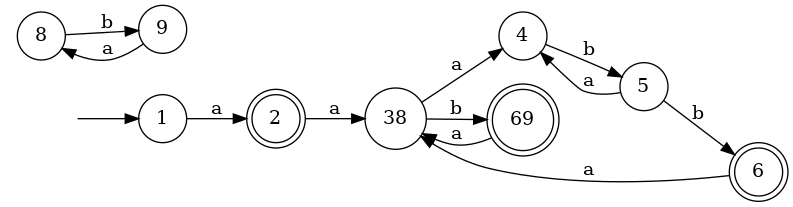
\includegraphics[width=1\textwidth]{pic3_2_2.dot}\\
    \end{center}
    Его можно минимизировать:
    \begin{center}
        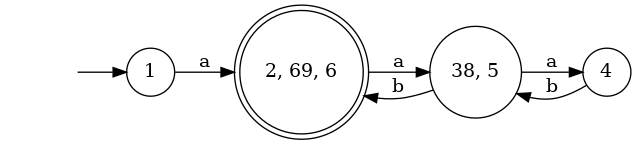
\includegraphics[width=1\textwidth]{pic3_2_3.dot}\\
    \end{center}
    
    3. $(a+(a+b)(a+b)b)*$\\
    Недетерминированный КА по данному выражению:
    \begin{center}
        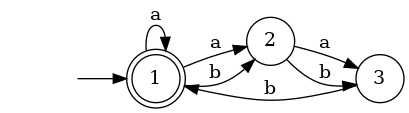
\includegraphics[width=0.6\textwidth]{pic3_3_1.dot}\\
    \end{center}
    \begin{center}
        \begin{tabular}{|c|c|c|}
            \hline
            Сочетания точек & По А & По В \\
            \hline
                1 & 12 & 2\\
                12 & 123 & 23\\
                2 & 3 & 3 \\
                3 &  & 1\\
                123 & 123 & 123 \\
                23 & 3 & 13 \\
                13 & 12 & 12 \\
            \hline
        \end{tabular}\\
    \end{center}
    Теперь можем нарисовать ДКА:
    \begin{center}
        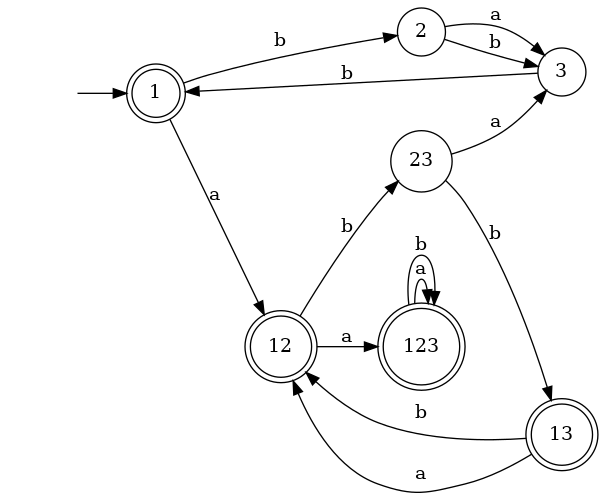
\includegraphics[width=1\textwidth]{pic3_3_2.dot}\\
    \end{center}
    Он минимален
    
    4. $(b+c)((ab)^*c+(ba)^*)^*$\\
    По счастливому стечению обстоятельств удаётся сразу построить ДКА:
    \begin{center}
        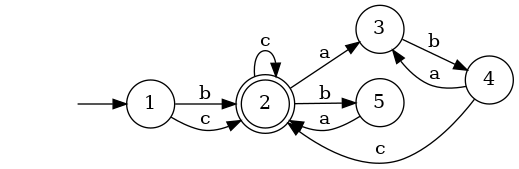
\includegraphics[width=1\textwidth]{pic3_4_1.dot}\\
    \end{center}
    Кажется, он еще и минимальный. Победа!
    
    5. $(a+b)^+(aa+bb+abab+baba)(a+b)^+$\\
    Недетерминированный КА по данному выражению:
    \begin{center}
        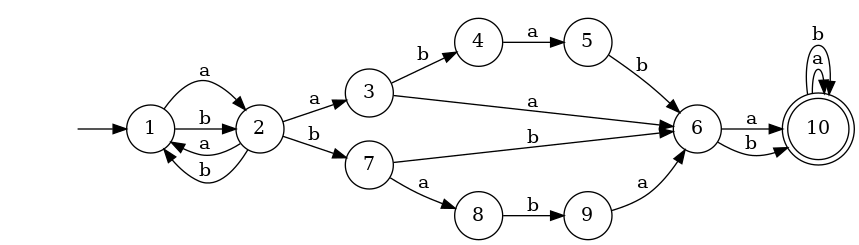
\includegraphics[width=1\textwidth]{pic3_5_1.dot}\\
    \end{center}
    \begin{center}
        \begin{tabular}{|c|c|c|}
            \hline
            Сочетания точек & По А & По В \\
            \hline
                1 & 2 & 2\\
                2 & 13 & 17\\
                13 & 26 & 24 \\
                17 & 28 & 26\\
                26 & 1310 & 1710 \\
                24 & 135 & 17 \\
                28 & 13 & 179 \\
                1310 & 2610 & 2410 \\
                1710 & 2810 & 2610 \\
                135 & 26 & 246 \\
                179 & 286 & 26 \\
                246 & 13510 & 1710 \\
                286 & 1310 & 17910 \\
                2610 & 1310 & 1710 \\
                2410 & 13510 & 1710 \\
                2810 & 1310 & 17910 \\
                13510 & 2610 & 24610 \\
                17910 & 28610 & 2610 \\
                24610 & 13510 & 1710 \\
                28610 & 1310 & 17910 \\
            \hline
        \end{tabular}\\
    \end{center}
    Теперь можем нарисовать ДКА:
    \begin{center}
        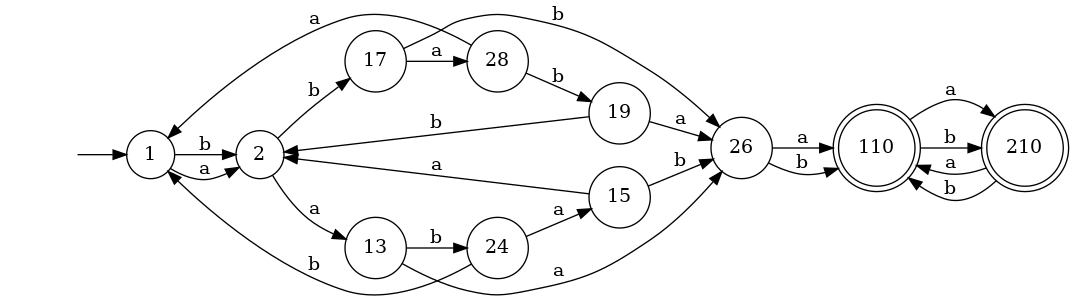
\includegraphics[width=1\textwidth]{pic3_5_2.dot}\\
    \end{center}
    Займёмся минимизацией:\\
    $0: \{1, 2, 13, 17, 26, 24, 28, 135, 179, 246, 286\}\{1310, 1710, 2610, ..., 28610\}$\\
    $1: \{1, 2, 13, 17, 24, 28, 135, 179\}\{26, 246, 286\}\{1310, 1710, 2610, ...,28610\}$\\
    $2: \{1, 2, 24, 28\}\{13\}\{17\}\{135, 179\}\{26, 246, 286\}\{1310, 1710, 2610, ...,28610\}$\\
    $3: \{1\}\{2\}\{24\}\{28\}\{13\}\{17\}\{135, 179\}\{26, 246, 286\}\{1310, 1710, 2610, ...,28610\}$\\
    \begin{center}
        \includegraphics[width=1\textwidth]{3_5}\\
    \end{center}
    Таким образом, получится автомат:
    \begin{center}
        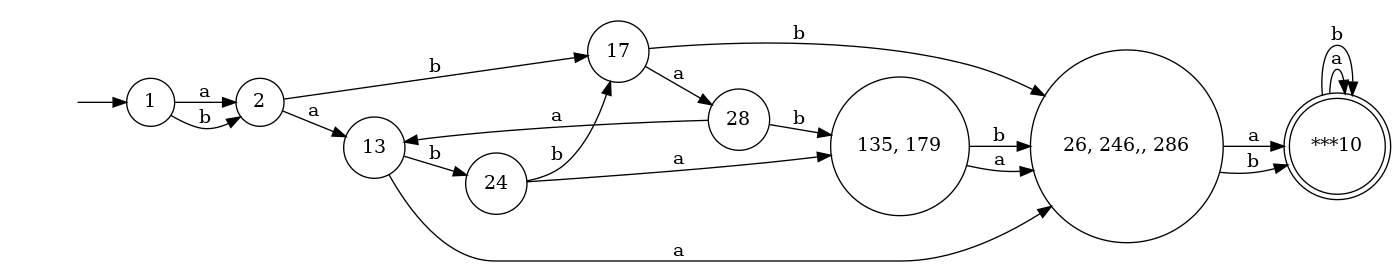
\includegraphics[width=1\textwidth]{pic3_5_3.dot}\\
    \end{center}
    
\section{Определить, является ли язык регулярным}
    1. $L=\{(aab)^nb(aba)^m \quad n \geq 0, m\geq 0\}$\\
    Можем построить КА:
    \begin{center}
        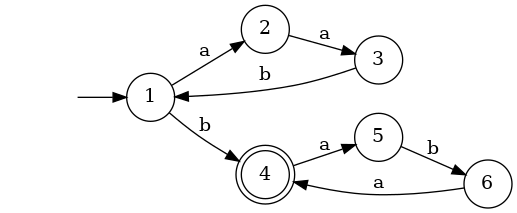
\includegraphics[width=0.6\textwidth]{pic4_1_1.dot}\\
    \end{center}
    
    2. $L=\{uaav \quad u \in \{a,b\}^*, v \in \{a,b\}^*, |u|_b \geq |v|_a\}$\\
    Пусть есть слово $w=b^naaa^n, |w|\geq n$.\\
    Разобьём на $w=xyz$, где $x=b^i, y=b^j, z=b^{n-i-j}aaa^n, |xy|\leq n, |y|>0$\\
    $w'=xy^kz = b^ib^{kj}b^{n-i-j}aaa^n$\\
    В случае $k=0$ имеем $w=b^{n-j}aaa^n$ и это слово не входит в язык $L$. Значит, по невыполнению теореме о разрастании, язык $L$ не регулярный.\\
    
    3. $L=\{a^mw \quad w\in \{a,b\}^*,1\leq|w|_b\leq m\}$\\
    Пусть есть слово $w=a^nb^n, |w|\geq n$.\\
    Разобьём на $w=xyz$, где $x=a^i, y=a^j, z=a^{n-i-j}b^n, |xy|\leq n, |y|>0$\\
    $w'=xy^kz = a^ia^{kj}a^{n-i-j}b^n$\\
    В случае $k=0$ имеем $w=a^{n-j}b^n$ и это слово не входит в язык $L$. Значит, по невыполнению теореме о разрастании, язык $L$ не регулярный.\\
    
    4. $L=\{a^kb^ma^n \quad k=n \vee m>0\}$\\
    Пусть есть слово $w=a^nba^n, |w|\geq n$.\\
    Разобьём на $w=xyz$, где $x=a^i, y=a^j, z=a^{n-i-j}ba^n, |xy|\leq n, |y|>0$\\
    $w'=xy^kz = a^ia^{kj}a^{n-i-j}ba^n$\\
    В случае $k=0$ имеем $w=a^{n-j}ba^n$ и это слово не входит в язык $L$. Значит, по невыполнению теореме о разрастании, язык $L$ не регулярный.\\
    
    5. $L=\{ucv \quad u\in\{a,b\}^*, v\in\{a,b\}^*, u \neq v^R\}$\\
    Пусть есть слово $w=(ab)^nc(ab)^n = \alpha_1\alpha_2...\alpha_{4n}\alpha_{4n+1}, |w|\geq n$.\\
    Разобьём на $w=xyz$, где\\ $x=\alpha_1\alpha_2...\alpha_{i}, \quad y=\alpha_{i+1}\alpha_{i+2}...\alpha_{i+j},\\ z=\alpha_{i+j+1}\alpha_{i+j+2}...\alpha_{2n}c(ba)^n, |xy|\leq n, |y|>0$\\
    $w'=xy^kz = (\alpha_1\alpha_2...\alpha_{i}) (\alpha_{i+1}\alpha_{i+2}...\alpha_{i+j})^k (\alpha_{i+j+1}\alpha_{i+j+2}...\alpha_{2n})c(ba)^n$\\
    В случае $k>1$ это слово не входит в язык $L$. Значит, по невыполнению теореме о разрастании, язык $L$ не регулярный.
\end{document}
